
%----------------------------------------------------------------------------------------
%	PACKAGES AND OTHER DOCUMENT CONFIGURATIONS
%----------------------------------------------------------------------------------------

\documentclass[paper=a4, fontsize=11pt]{scrartcl} % A4 paper and 11pt font size

\usepackage[T1]{fontenc} % Use 8-bit encoding that has 256 glyphs
\usepackage{fourier} % Use the Adobe Utopia font for the document - comment this line to return to the LaTeX default
\usepackage[UTF8]{inputenc}
\usepackage[english]{babel} % English language/hyphenation
\usepackage{amsmath,amsfonts,amsthm} % Math packages

\usepackage{listings}
\usepackage{courier}
\lstset{basicstyle=\footnotesize\ttfamily,breaklines=true}
\lstset{language=Python}
\lstset{frame=topbottom,stepnumber=5,numbers=left}

\usepackage{lipsum} % Used for inserting dummy 'Lorem ipsum' text into the template

\usepackage{graphicx}

\usepackage{sectsty} % Allows customizing section commands
\allsectionsfont{\centering \normalfont\scshape} % Make all sections centered, the default font and small caps

\usepackage{fancyhdr} % Custom headers and footers
\pagestyle{fancyplain} % Makes all pages in the document conform to the custom headers and footers
\fancyhead{} % No page header - if you want one, create it in the same way as the footers below
\fancyfoot[L]{} % Empty left footer
\fancyfoot[C]{} % Empty center footer
\fancyfoot[R]{\thepage} % Page numbering for right footer
\renewcommand{\headrulewidth}{0pt} % Remove header underlines
\renewcommand{\footrulewidth}{0pt} % Remove footer underlines
\setlength{\headheight}{13.6pt} % Customize the height of the header

\numberwithin{equation}{section} % Number equations within sections (i.e. 1.1, 1.2, 2.1, 2.2 instead of 1, 2, 3, 4)
\numberwithin{figure}{section} % Number figures within sections (i.e. 1.1, 1.2, 2.1, 2.2 instead of 1, 2, 3, 4)
\numberwithin{table}{section} % Number tables within sections (i.e. 1.1, 1.2, 2.1, 2.2 instead of 1, 2, 3, 4)

\setlength\parindent{0pt} % Removes all indentation from paragraphs - comment this line for an assignment with lots of text

%----------------------------------------------------------------------------------------
%	TITLE SECTION
%----------------------------------------------------------------------------------------

\newcommand{\horrule}[1]{\rule{\linewidth}{#1}} % Create horizontal rule command with 1 argument of height

\title{	
\normalfont \normalsize 
\textsc{University of Twente --- Applied Mathematics} \\ [25pt] % Your university, school and/or department name(s)
\horrule{0.5pt} \\[0.4cm] % Thin top horizontal rule
\huge Random Signals \& Filtering --- Practical \\ % The assignment title
\horrule{2pt} \\[0.5cm] % Thick bottom horizontal rule
}

\author{Hidde Wieringa (s1343041)} % Your name
\date{\normalsize\today} % Today's date or a custom date

\newcommand{\diff}{\,\text{d}}

\begin{document}

\maketitle % Print the title

\newpage 
\section{Mathematics}

In the following section I will describe all mathematical modelling required for the (Extended) Kalman filter and Particle filter to work correctly. 

For this assignment we consider a signal model of the form 
\begin{eqnarray}\label{eq:2}
	x_{k+1} &=& f(x_k) + w_k,\\
	y_{k} &=& h(x_k) + v_k.
\end{eqnarray}
We assume $k \geq 0$. The known functions $f$ and $h$ must be differentiable once in any reachable point $x_k$. The first state $x_0 \sim X_0 =N(\mu, \sigma^2)$, all $\{w_k\} \sim N(0,Q^2)$ and all $\{v_k\} \sim N(0,R^2)$. Also all $x_0$, $\{w_k\}$ and $\{v_k\}$ are independent. Below are the algorithms for the (Extended) Kalman filter and the Particle filter. 

Only scalar functions and values are considered in this assignment, although any theory and code can be trivially extended to a more general, multi-dimensional form.

Data for the the system can be generated in the following way:
		
\subsection{Generating data}

Sample data is crucial for testing and comparing signal filters. For the model above, I generated data using the following algorithm:
\begin{enumerate}
	\item Initialize a variable $x_0$ by drawing from the $X_0$ distribution. Let $k=0$. 
	\item Draw two independent random variables $v\sim N(0,Q^2)$ and $w\sim N(0,R^2)$.
	\item Let $x_{k+1}$ be $f(x_{k})+w$.
	\item Let $y_{k}$ be $h(x_{k})+v$.
	\item Increase $k$ by 1.
	\item Repeat from step b) until no more observations $y_k$ are required.
\end{enumerate}

For the first state of the system, $x_0$, an observation $y_0$ is created. Usually only the observations $y_k$ need to be outputted and only the last state $x_k$ needs to be stored. However, to compare data and plot the results, it is useful to store all $x_k$ and $y_k$.


\subsection{(Extended) Kalman filter}

For the Extended Kalman Filter the known functions $f$ and $h$ are approximated by a Tailor series to make the model linear in $x_k$. This results in the Jacobians of $f$ and $h$ being used in the algorithm. They are defined by
$$
F_k=f'(x_k),\qquad H_k=h'(x_k).
$$
It is easy to find that the normal Kalman filter is an instance of the Extended Kalman filter where 
\begin{eqnarray*}
	f(x) &=& Fx,\\
	h(x) &=& Hx
\end{eqnarray*}
where $F$ and $H$ can be matrices, but are scalars in the scope of this assignment. This means that the Jacobians of $f$ and $h$ are respectively $F$ and $H$. 

The filter consists of a few algorithmic steps:
\begin{enumerate}
	\item Initialize $x_0$ and $\Sigma_0$ by letting them be $E(X_0)$ and $\text{cov}(X_0)$ respectively. Let $k$ be $0$.
	\item Time update:
	\begin{enumerate}
		\item Let $x_{k+1}$ be $f(x_k)$. 
		\item Let $\Sigma_{k+1}$ be $F_k \Sigma_k F_k+Q$. 
	\end{enumerate}
	\item Let $S_k$ be $H_k\Sigma_kH_k+R$ and $K_k$ be $\Sigma_kH_k/S$.
	\item Measurement update:
	\begin{enumerate}
		\item Add $K_k(y_k-h(x_{k+1}))$ to $x_{k+1}$. 
		\item Multiply $\Sigma_{k+1}$ by $1-K_k H_k$. 
	\end{enumerate}
	\item Increase $k$ by 1.
	\item Repeat from step 2 for each new observation.
\end{enumerate}

These calculations are simple additions and multiplications for each new observation. No distributions need to be drawn from and no PDF or CDF functions need to be known throughout the filtering process.

\subsection{Particle filter}

For the Particle filter there are two parameters to be chosen, namely $N$ and $T$. The number of particles is determined by $N$. The value of $T$ defines the threshold when a resampling is done. When $T=0$, no resampling is done. Whenever $T=1$ a resample is done each iteration of the filter. 

For the proposal distribution $\pi(\cdot)$ is chosen to be $p(x_k^i|x_{k-1}^i)$. This makes drawing from it easy (used in the time update step). The weight update step becomes $$
w_{k+1}^i=w_{k}^i\frac{p(y_k|x_k^i)p(x_k^i|x_{k-1}^i)}{\pi(x_{0:k},y_k)}=w_{k}^ip(y_k|x_k^i).
$$

Below are the algorithmic steps for the Particle filter:
\begin{enumerate}
	\item Initialize $N$ particles $x_0^i$ with weights $1/N$ by drawing from $N$ samples from the $X_0$ distribution. Let $k$ be $1$.
	\item Time update:
	\begin{enumerate}
		\item Draw $N$ independent random $v^i \sim N(0,Q^2)$ for all $i=1,...,N$.
		\item Let $x_{k+1}^i$ be $f(x_{k}^i)+v^i$ for all $i=1,...,N$.
	\end{enumerate}
	\item Measurement update: 
	\begin{enumerate}
		\item Calculate the weights $w_{k+1}^i$ using $
	w_{k+1}^i=w_{k}^ip(y_k|x_k^i)$.
	At the same time, keep track of the sum $S = \sum_{i=1}^N w_{k+1}^i$.
		\item Divide $w_{k+1}^i$ by $S$ to normalize the weights for all $i=1,...,N$.
	\end{enumerate}
	\item Calculate $N_\text{eff}=\left(\sum_{i=1}^N \left(w_{k+1}^i\right)^2\right)^{-1}.$ If $N_\text{eff} < NT$, resample the particles:
	\begin{enumerate}
		\item Draw $N$ new particles from the discrete distribution $x_{k+1}^i$ with weights $w_{k+1}^i$, and give them weights $1/N$.
	\end{enumerate}
	\item Increase $k$ by 1.
	\item Repeat from step 2 for each new observation.
\end{enumerate}

Because the relation between $y_k$ and $x_{k}$ is
$$
y_k=h(x_k) +v_k,
$$
and $x_k$ is assumed known, the distribution $p(y_k|x_k^i)$ is a shifted normal distribution $N\left(h(x_k^i),R^2\right)$. This means that the only the PDF function of $N\left(h(x_k^i),R^2\right)$ needs to be known for all $i=1,...,N$.

The expected value of $x_{k+1}$ given all previous data can be calculated using $$
\hat{x}_{k+1} = E(x_{k+1}|x_{0:k},y_{0:k})=\sum_{i=1}^N w_{k+1}^i x_{k+1}^i.
$$
The mean squared error can be found using the standard formula for the variance of a distribution $$
\text{var}(X) = E\left((X - E(X))^2\right),
$$
in our case the approximation
\begin{equation}\label{eq:1}
\text{var}(x_{k+1}|x_{0:k},y_{0:k}) \approx \sum_{i=1}^N w_{k+1}^i \left(x_{k+1}^i-\hat{x}_{k+1}\right)^2.
\end{equation}

\section{Linear model}

For this assignment the following instance of the base model (\ref{eq:2}) is used:
\begin{eqnarray*}
	f(x) = x \qquad F_k = 1 \qquad Q = 1 \\
	h(x) = x \qquad H_k = 1 \qquad R = 1 \\
	\mu = 10 \qquad \sigma = 1
\end{eqnarray*}

\subsection{Parameters}

\begin{figure}
\centerline{
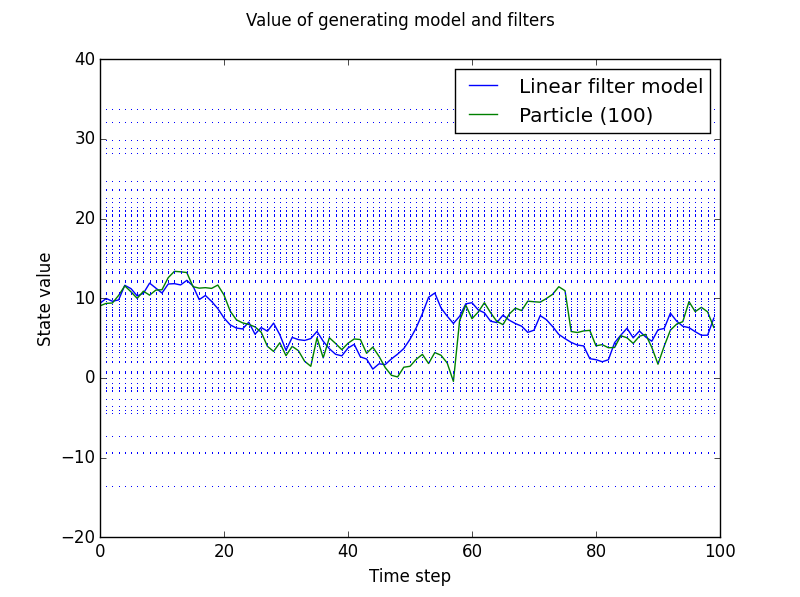
\includegraphics[width=.7\textwidth]{fig/figure_5}
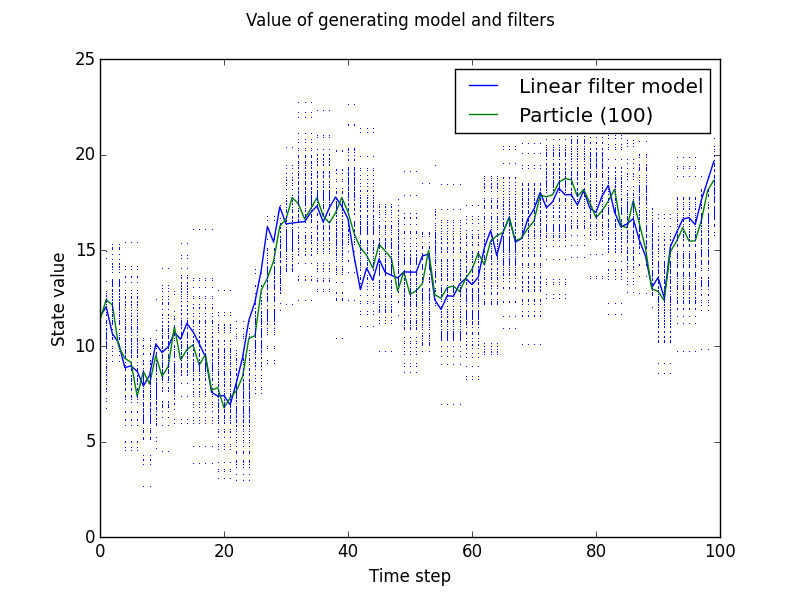
\includegraphics[width=.7\textwidth]{fig/figure_6}}
\centerline{
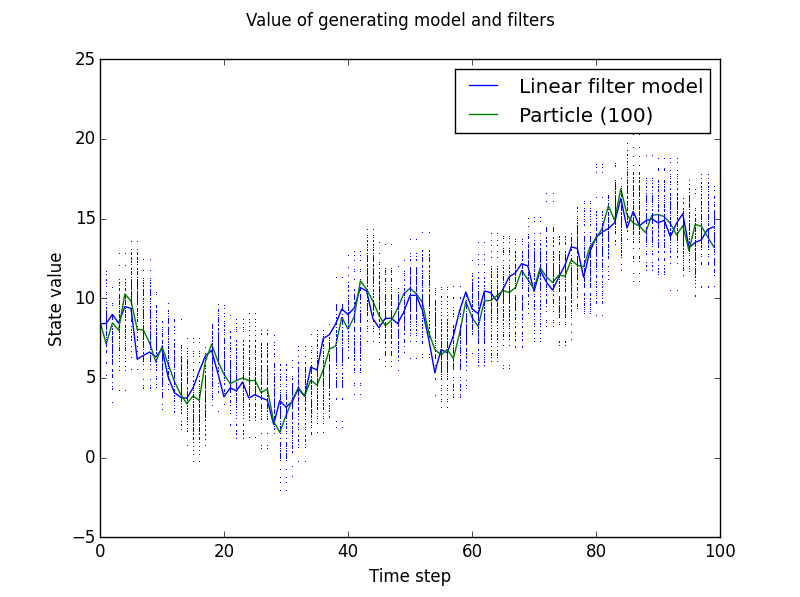
\includegraphics[width=.7\textwidth]{fig/figure_7}
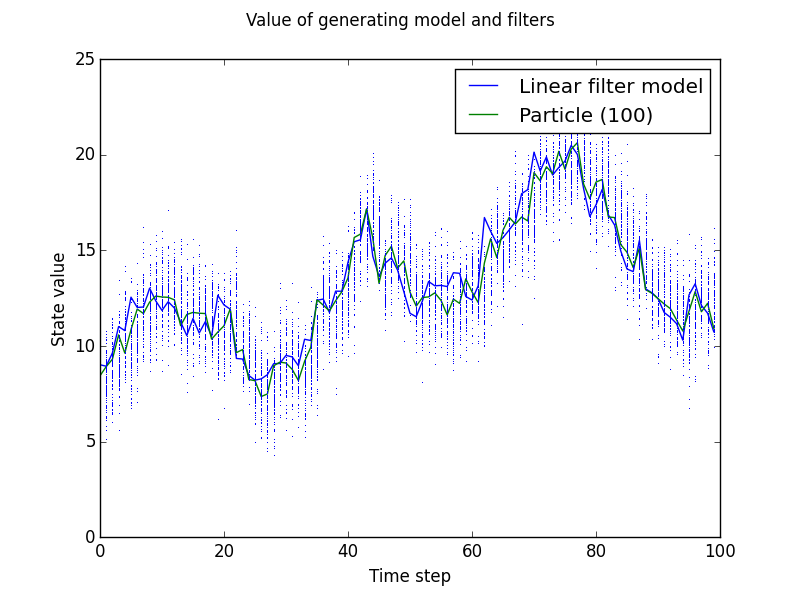
\includegraphics[width=.7\textwidth]{fig/figure_8}}
\caption{Particle filter with values for $T$ in $\{0, 1/3, 2/3, 1\}$.}\label{fig:3}
\end{figure}

The value of $T$ has been chosen as 1. This means a resample the particles is done every iteration of $k$. In figure \ref{fig:3} a comparison is made between a few values of $T$. The Particle filter works worse when a low $T$ is chosen, because of particle impoverishment. Almost no difference is seen in the error between $T=2/3$ and $T=1$, but because the filters are very quick extra resampling is not a problem. 

The value of $N$ is chosen as $100$. This number of particles gives very quick filtering results and approximates the values for $x_k$ almost in distinctive from the Kalman filter which is optimal.

\subsection{MSE}

The mean squared error of the Particle filter can be calculated using (\ref{eq:1}).

\subsection{MSE against actual error}

When comparing the MSE against the actual error from the truth data, two things require attention.

The average of the actual error seems to be approximated well by the MSE calculated by the Kalman and Particle filters. Of course the actual error is sometimes larger and sometimes smaller than the MSE. This is because of the noise on the measurement data. The filters do not follow the measurements one-to-one to guess the state, because a change in the measurement could also mean an error instead of a change of the state. 

When the measurements structurally differ from the guessed state, the change must be a state change so the state guess of the filters gets updated.

Secondly, as $N$ grows, the Kalman and Particle filters become practically equivalent. The same state is guessed by both filters and the same guess error (actual error from the truth value) is made.

\begin{figure}
\centerline{
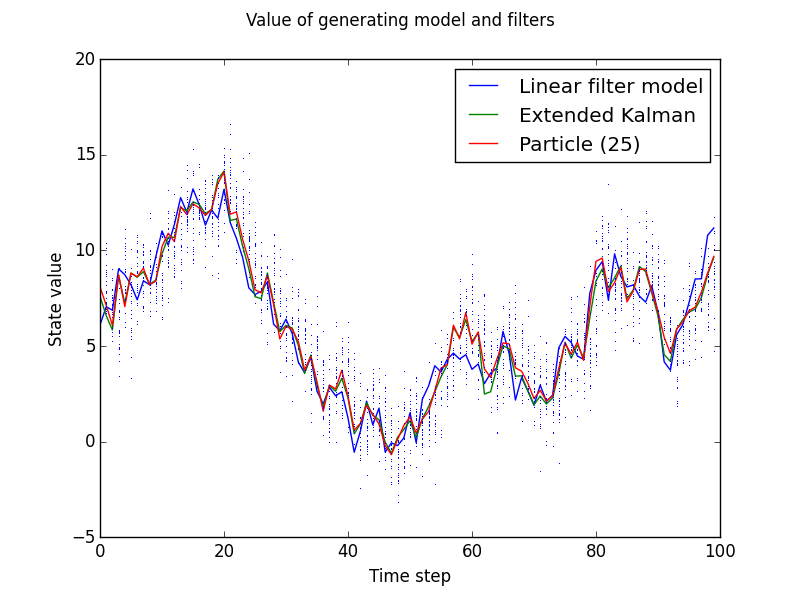
\includegraphics[width=.7\textwidth]{fig/figure_1}
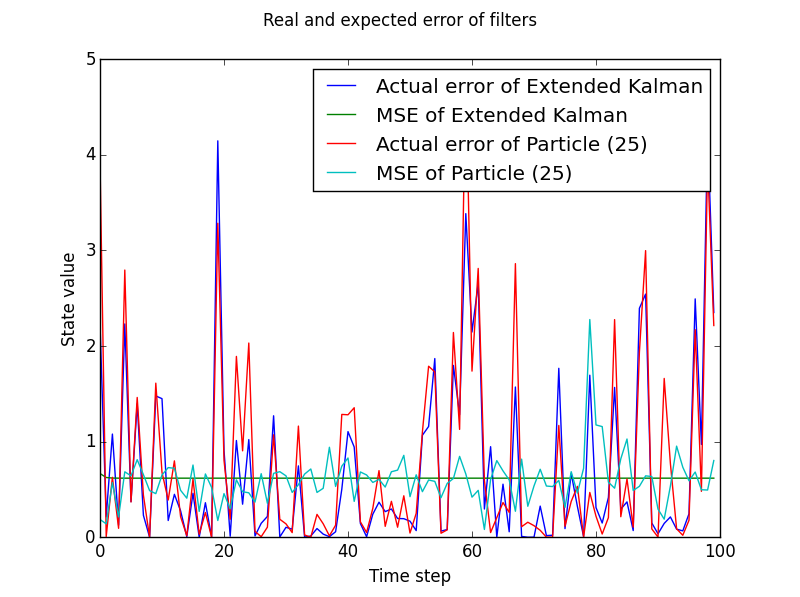
\includegraphics[width=.7\textwidth]{fig/figure_2}}
\caption{Linear Kalman filter and Particle filter with $N=25$.}\label{fig:1}
\end{figure}
\begin{figure}
\centerline{
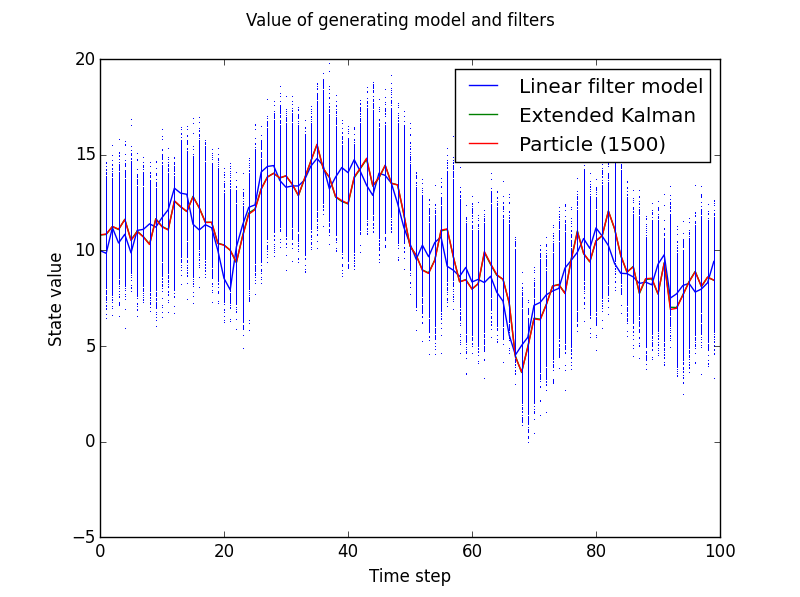
\includegraphics[width=.7\textwidth]{fig/figure_3}
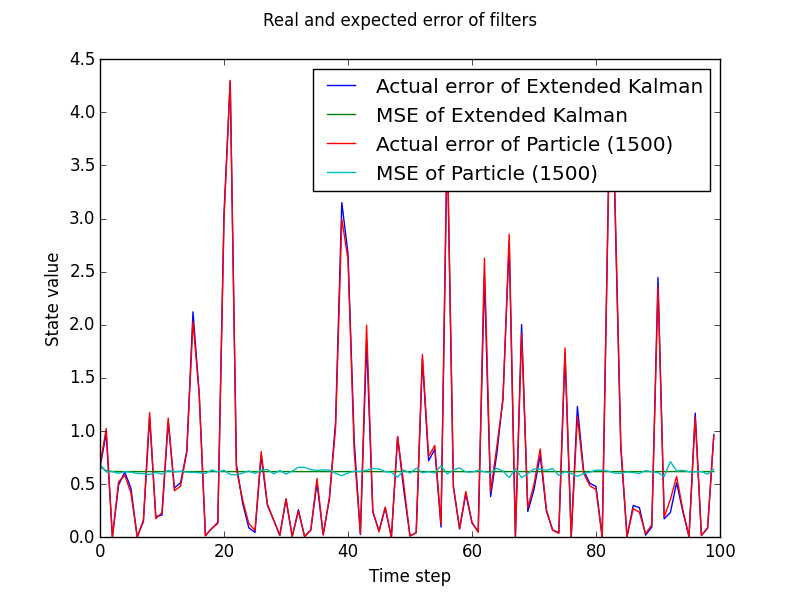
\includegraphics[width=.7\textwidth]{fig/figure_4}}
\caption{Linear Kalman filter and Particle filter with $N=1500$.}\label{fig:2}
\end{figure}


\subsection{Number of particles}

In figure \ref{fig:1} and figure \ref{fig:2} we can see the difference between the Kalman filter and the Particle filter. Only the images for $N=25$ and $N=1500$ are displayed here. Any value for $N$ in between gives results between the two extremes.

Two things are interesting. First of all the MSE of the Kalman filter converges quickly to a single value. On average, the MSE of the Particle filter is the same value (although it does not seem to converge to it). For a larger $N$, the MSE of the Particle filter does not become smaller. This is logical, because the error introduced by the measurement noise does not become less.

Secondly I see that for a larger value of $N$, the distribution the particles of the Particle filter represent, converge closer to the actual distribution of the state $x_k$. This means that the approximation of the state $x_k$ becomes better: the MSE of the Particle filter is closer to the MSE of the Kalman filter. In the image on the left there is practically no difference between the expected $x_k$ of the Kalman and Particle filter.

This result is expected: The Kalman filter has the minimum possible squared error, so is optimal. The Particle filter will approach the perfect distribution as $N \rightarrow \infty$. Together this means that no better approximation of the state $x_k$ is possible for this model.

\subsection{Variation of data}

\begin{figure}
\centerline{
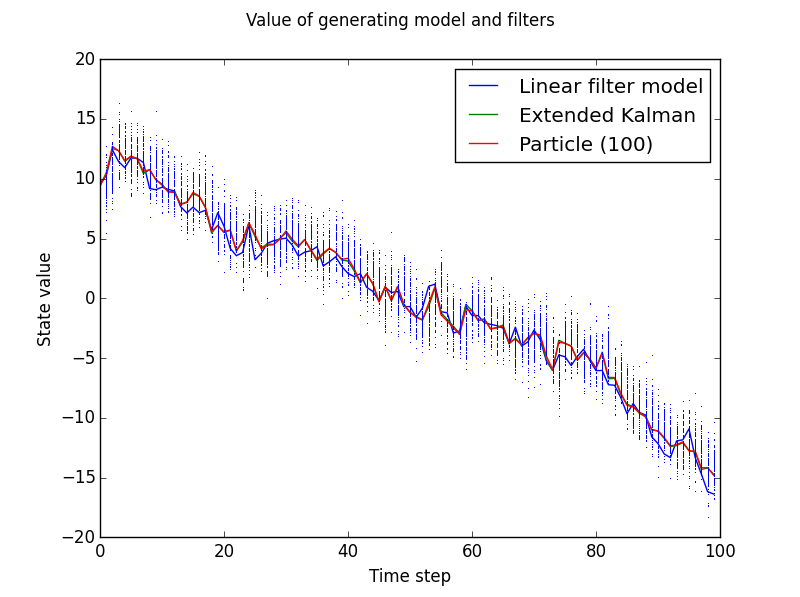
\includegraphics[width=.7\textwidth]{fig/figure_9}
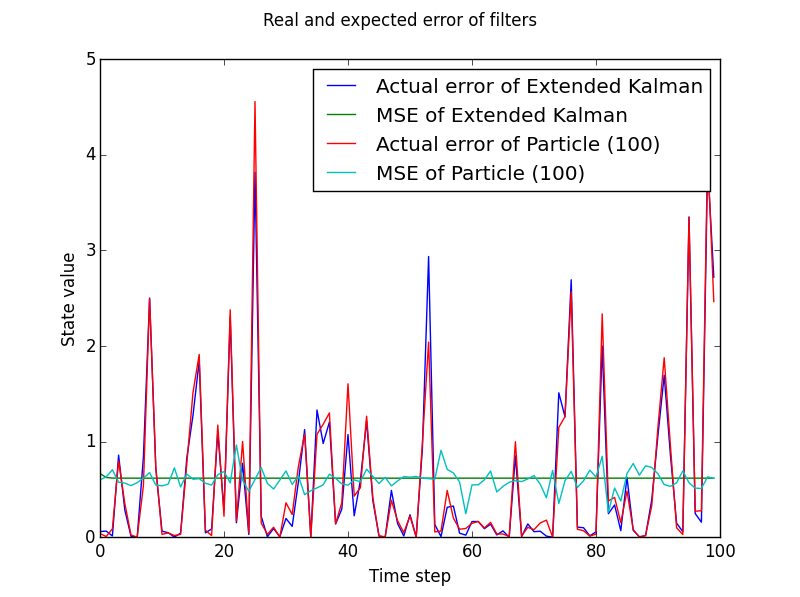
\includegraphics[width=.7\textwidth]{fig/figure_10}}
\centerline{
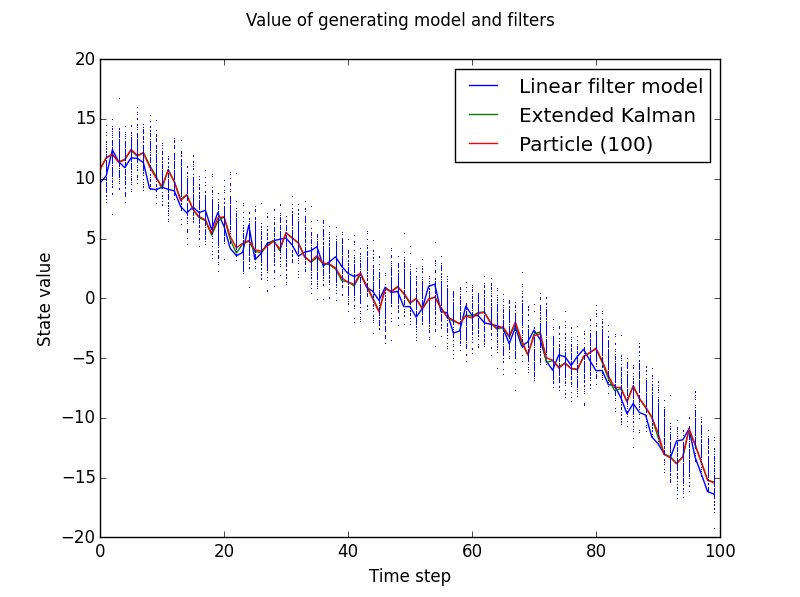
\includegraphics[width=.7\textwidth]{fig/figure_11}
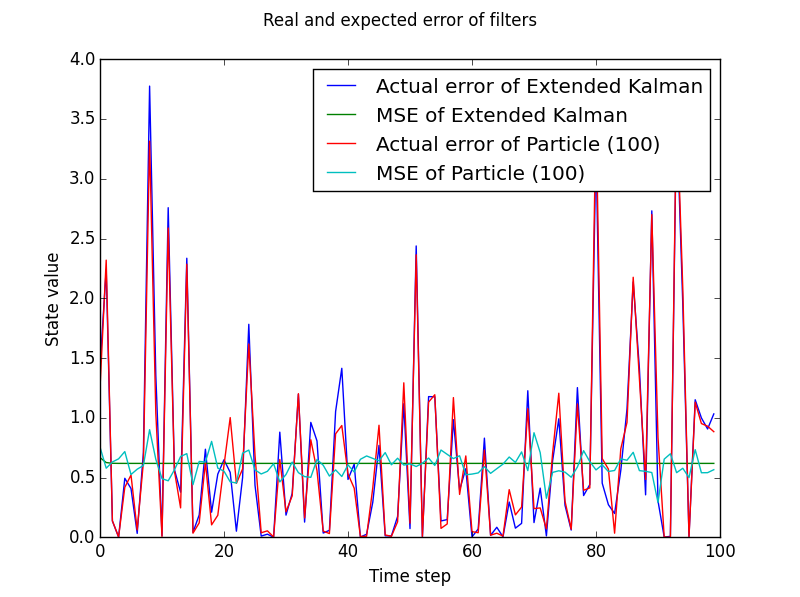
\includegraphics[width=.7\textwidth]{fig/figure_12}}
\caption{Filtering of a variation of data, with the same truth.}\label{fig:4}
\end{figure}

When the same truth is used, but different data is generated because of different measurement noise, the filters give a different guess for the state $x_k$. See figure \ref{fig:4} for two comparisons.

Because the filters do not know that the same truth is being used, no extra information can be retrieved from the data by the filter to give a better prediction.

\section{Nonlinear model}

For this assignment the following instance of the base model (\ref{eq:2}) is used:
\begin{eqnarray*}
	f(x) = \sin(x) \qquad F_k = \cos(x_k) \qquad Q = 1 \\
	h(x) = \cos(x) \qquad H_k = -\sin(x_k) \qquad R = 1 \\
	\mu = 10 \qquad \sigma = 1
\end{eqnarray*}

\subsection{MSE against actual error}

\begin{figure}
\centerline{
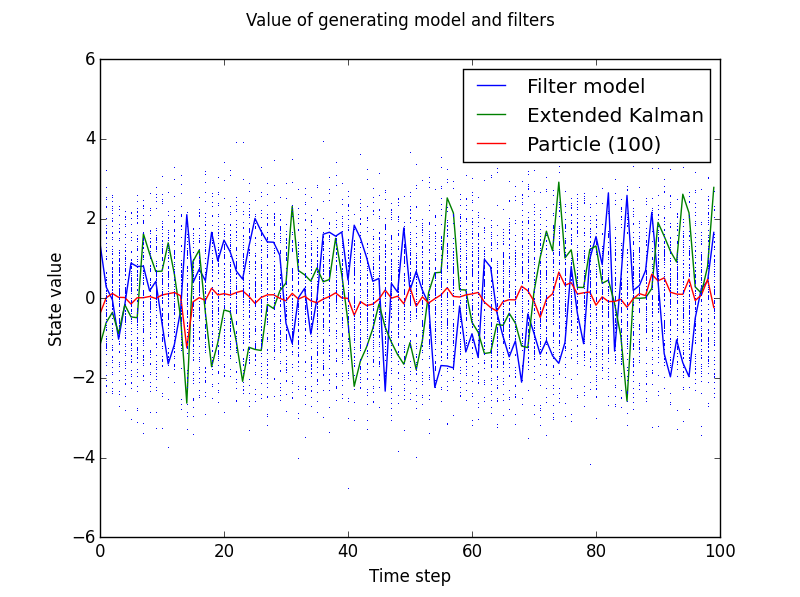
\includegraphics[width=.7\textwidth]{fig/figure_13}
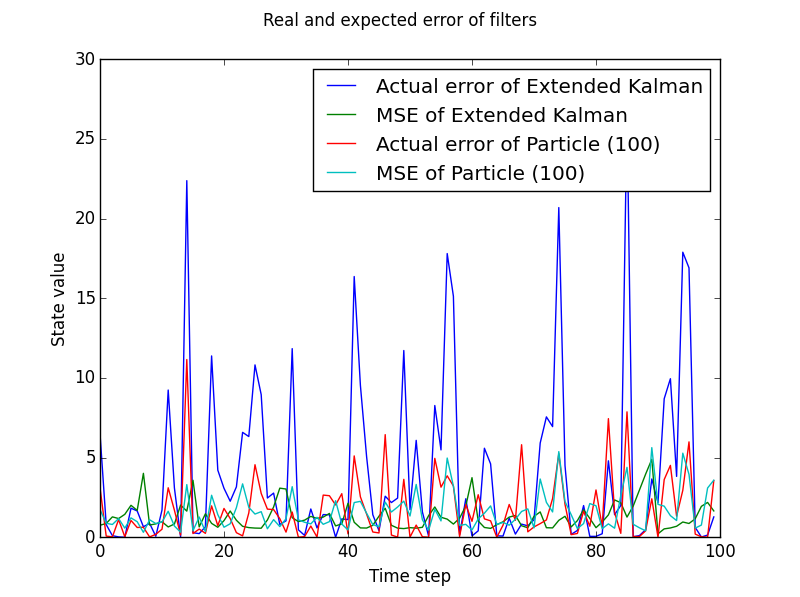
\includegraphics[width=.7\textwidth]{fig/figure_14}}
\caption{Filtering of nonlinear model.}\label{fig:5}
\end{figure}

In figure \ref{fig:5} the filtering of the nonlinear model can be seen. The errors, both the MSE and actual errors from the truth data are gigantic. They do not improve over time(steps). The Kalman filters models either the truth or the negative version of the truth.

First the Kalman filter. It has a single guessed state $x_k$ stored, which it updates based on observations. For these observations, both $x_{k+1}$ and $-x_{k+1}$ are valid, because $\cos(x)=\cos(-x)$. The Kalman filter will try to follow the positive or negative state, based on the noise (which of the two seems more likely).

The Particle filter has many possible states $x_k^i$ stored, which represent the distribution of the state together. However, just like with the Kalman filter, both the positive and negative variants of the state are both probable. Because the noise is also symmetric around zero (normal distribution), and neither variant (positive or negative) of the particles will receive a smaller weight. The result is a distribution which has an expectation equal to zero, and a large variance.

To verify the observations above, I changed the parameters of the model. Two simulations can be found in figure \ref{fig:6}. The new parameters are $Q=0.1$, $R=0.2$ and $\mu=0.5$. The result of the change of parameters are three things. The initial value is small (around 0.5) which makes the reasoning about the model simpler. The change of the state is reduced such that it becomes smoother. The noise on the observations becomes much smaller to be able to observe the state better for the filters.

In the figure it is easy to see the symmetric distribution of the state. The Kalman filter sometimes follows the state and sometimes follows the negative state. Changes of which state is followed by the filter occur whenever the change of the state was large.

The Particle filter follows both the positive and negative state with its particles. This means that the average becomes zero after a while. It is interesting to see that in figure \ref{fig:6} (left) the particles have a peak when the state diverges from zero. This is because the information that the initial value of the state is positive is used and the positive state is the more probable of the two.

\begin{figure}
\centerline{
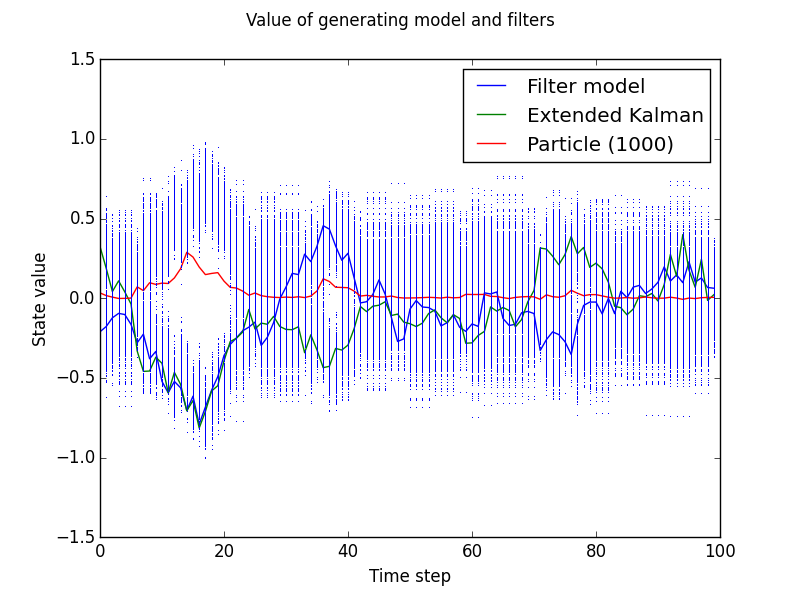
\includegraphics[width=.7\textwidth]{fig/figure_15}
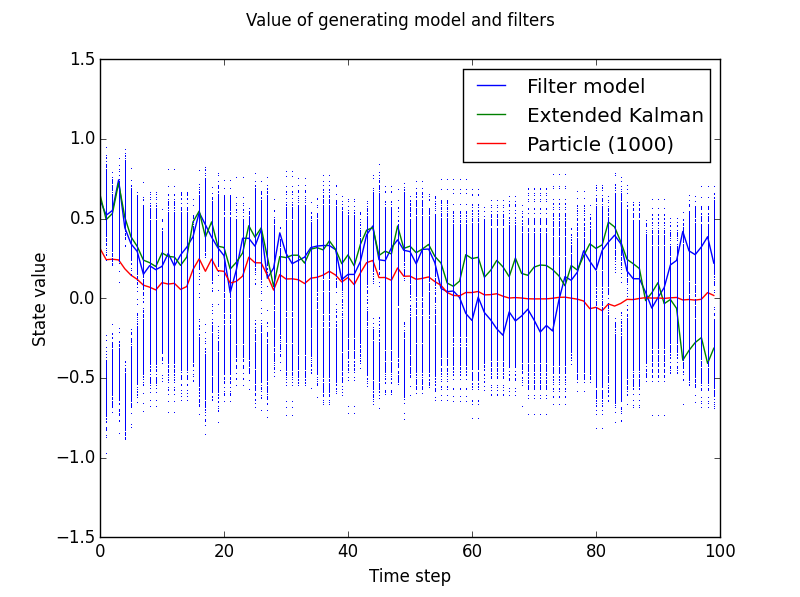
\includegraphics[width=.7\textwidth]{fig/figure_16}}
\caption{Symmetric filtering of nonlinear model with little measurement noise ($Q=0.1$, $R=0.02$ and $\mu=0.5$).}\label{fig:6}
\end{figure}

\subsection{Number of particles}

As observed in the linear model, when more particles are used the actual distribution of the state is better represented by the particles.

For this model, when more particles are used, the quicker the particle filter converges to zero. Also, with more particles it is easier to visualize what is going on in the filter because the distribution is more clear.

For this reason the initial number of particles used was 100, but for the detailed investigation I used 1000 particles.

\subsection{Variation of data}

\begin{figure}
\centerline{
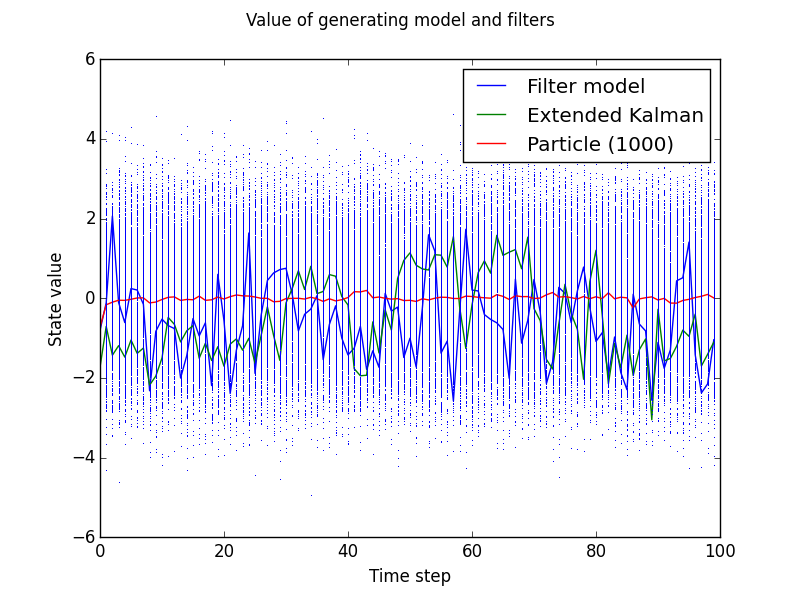
\includegraphics[width=.7\textwidth]{fig/figure_17}
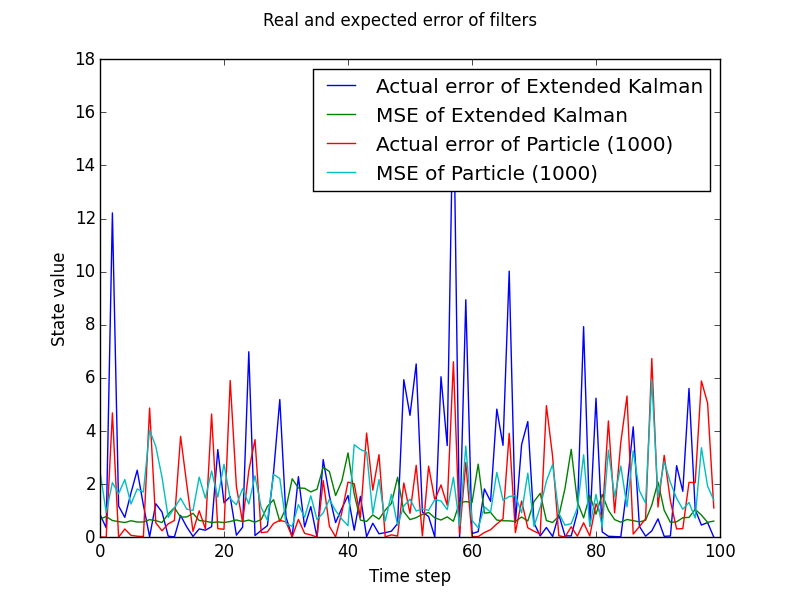
\includegraphics[width=.7\textwidth]{fig/figure_18}}
\centerline{
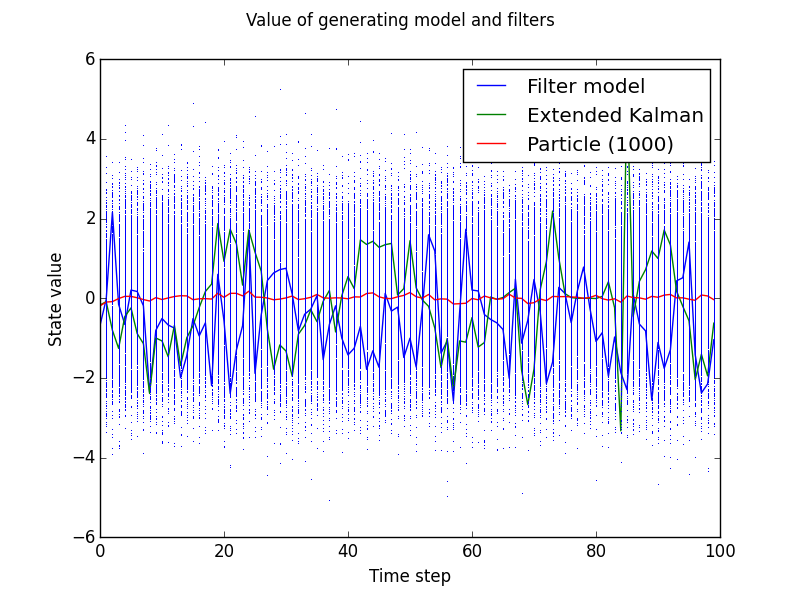
\includegraphics[width=.7\textwidth]{fig/figure_19}
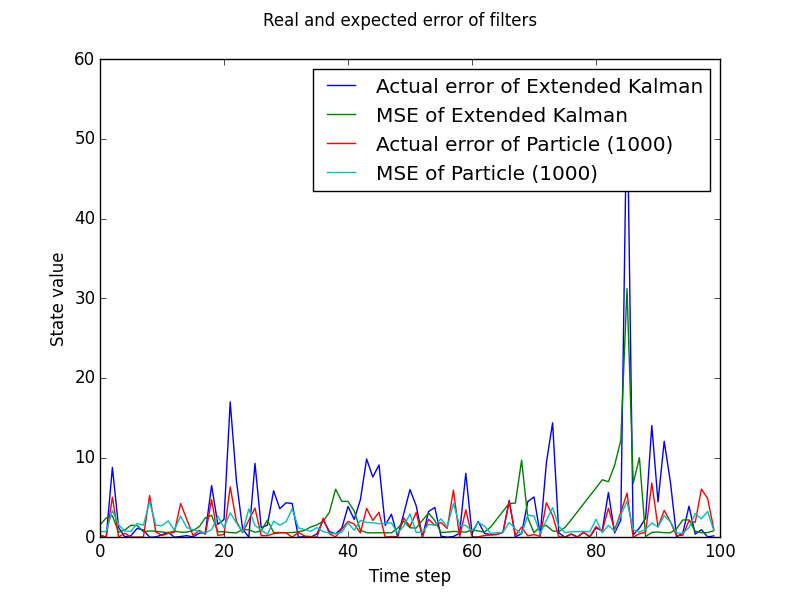
\includegraphics[width=.7\textwidth]{fig/figure_20}}
\caption{Filtering of a variation of data, with the same truth.}\label{fig:6}
\end{figure}

The results are the same as for the linear model.
When the same truth is used, but different data is generated because of different measurement noise, the filters give a different guess for the state $x_k$. See figure \ref{fig:6} for two comparisons.

Because the filters do not know that the same truth is being used, no extra information can be retrieved from the data by the filter to give a better prediction. The same symmetric filter properties apply for the same truth: based on the measurement noise the Kalman filter changes from the positive to negative state. 

\section{Implementation}

All implementation is done using the programming language Python. For the visualisation of the data and results the libraries NumPy and MatPlotLib are used.

The implementation is divided into four parts:
\begin{enumerate}
	\item Distributions:
	
	A basic object layout is used for each distribution. The properties expectation, variance and the PDF and CDF functions are implemented. Also, when possible, one can draw from the distribution.
	
	The normal, noise ($N(0, \sigma^2)$), uniform, static (zero variance) and discrete distributions are implemented.
	
	\item Models:
	
	A basic model class is implemented which stores information about $X_0$, the distribution of $w$ and $v$, the $f$ and $h$ functions and their Jacobians $F$ and $H$. Each model can generate data.
	
	A linear model class can be used for linear models which only requires the $X_0$, $w$ and $v$ distributions and the $F$ and $H$ values.
	
	\item Filters:
	
	Three filters are implemented. The Extended Kalman filter filters data for non-linear models. The basic Kalman filter filters data for linear models and uses the Extended Kalman filter internally. Finally, the Particle filter will use a configurable number of particles and resample threshold for its filter.
	
	Each of the filters is created in such a way that if new measurements comes in while the program is running, the filter can be updated with the new measurements. This means only a small state is stored in each filter.
	
	For visualisation purposes these implementations store all information instead of only the minimal state. 
	
	\item Main program:
	
	This runs the code which builds the models, generates data, filters the data and plots the results.
	
	
\end{enumerate}

\newpage
\section*{Appendix: code}

Distributions, \textit{distribution.py}:
\begin{lstlisting}

import random


class Distribution:

    def expectation(self):
        raise NotImplementedError

    def variance(self):
        raise NotImplementedError

    def draw(self):
        raise NotImplementedError

    def pdf(self, x):
        raise NotImplementedError

    def cdf(self, x):
        raise NotImplementedError


class NormalDistribution (Distribution):
    def __init__(self, mu, sigma):
        assert sigma > 0
        self.mu = mu
        self.sigma = sigma

    def expectation(self):
        return self.mu

    def variance(self):
        return self.sigma ** 2

    def draw(self):
        return random.normalvariate(self.mu, self.sigma)

    def pdf(self, x):
        return math.exp(- (x - self.mu) ** 2 / (2 * self.sigma ** 2)) / (self.sigma * math.sqrt(2 * math.pi))

    def cdf(self, x):
        raise NotImplementedError


class NoiseDistribution (NormalDistribution):
    def __init__(self, sigma):
        super().__init__(0, sigma)

    def cdf(self, x):
        raise NotImplementedError


class DiscreteDistribution (Distribution):
    def __init__(self, values):
        s = sum(w for (x, w) in values)
        assert s > 0
        # Normalize weights
        for i in range(len(values)):
            values[i][1] /= s

        self.values = values
        self.U = UniformDistribution(0, 1)

    def expectation(self):
        return sum(w * x for (x, w) in self.values)

    def variance(self):
        e = self.expectation()
        return sum(w * (x - e) ** 2 for (x, w) in self.values)

    def draw(self):
        u = self.U.draw()
        s = 0
        for (x, w) in self.values:
            if s + w > u:
                return x
            s += w
        raise NotImplementedError

    def pdf(self, x):
        raise NotImplementedError

    def cdf(self, x):
        raise NotImplementedError


class UniformDistribution (Distribution):
    def __init__(self, a, b):
        assert a < b
        self.a = a
        self.b = b

    def expectation(self):
        return (self.b + self.a) / 2

    def variance(self):
        return (self.b - self.a) ** 2 / 12

    def draw(self):
        return random.uniform(self.a, self.b)

    def pdf(self, x):
        if self.a <= x <= self.b:
            return 1 / (self.b - self.a)
        return 0

    def cdf(self, x):
        if x < self.a:
            return 0
        if x <= self.b:
            return (x - self.a) / (self.b - self.a)
        return 1


class StaticDistribution (Distribution):
    def __init__(self, q):
        self.q = q

    def expectation(self):
        return self.q

    def variance(self):
        return 0

    def draw(self):
        return self.q

    def pdf(self, x):
        if x == self.q:
            return float('inf')
        return 0

    def cdf(self, x):
        if x < self.q:
            return 0
        return 1

\end{lstlisting}

Models, \textit{model.py}:
\begin{lstlisting}

from distribution import *


class FilterModel:
    def __init__(self, X0: Distribution, V: NoiseDistribution, W: NoiseDistribution, f, F, h, H):
        self.xs = []
        self.ys = []
        self.k = 0

        self.X0 = X0
        self.f = f
        self.F = F
        self.h = h
        self.H = H

        # Generate x0
        self.x = X0.draw()
        self.y = None

        self.V = V
        self.W = W

    def generate(self):
        """
        Given self.x = x_k, generate x_{k+1} = x_k + v_k and y_k = x_k + w_k
        """
        self.x = self.f(self.x) + self.V.draw()
        self.y = self.h(self.x) + self.W.draw()

        self.xs.append(self.x)
        self.ys.append(self.y)

        self.k += 1

        return self.y

    @property
    def name(self):
        return 'Filter model'


class LinearFilterModel(FilterModel):
    def __init__(self, X0: Distribution, V: NoiseDistribution, W: NoiseDistribution, F, H):
        super().__init__(X0, V, W, lambda x: F * x, lambda _: F, lambda x: H * x, lambda _: H)

    @property
    def name(self):
        return 'Linear filter model'


\end{lstlisting}

Filters, \textit{filter.py}:
\begin{lstlisting}


from model import *


class Filter:
    """ Base abstract filter class """
    def __init__(self):
        """ Default constructor """
        self.k = 0
        self.xs = []
        self.mses = []

    def update(self, y):
        """ Process a new observation """
        raise NotImplementedError()

    @property
    def name(self):
        raise NotImplementedError()


class ExtendedKalmanFilter(Filter):
    def __init__(self, model: FilterModel):
        super().__init__()

        self.x = model.X0.expectation()
        self.sig = model.X0.variance()

        self.Q = model.V.variance()
        self.R = model.W.variance()
        self.f = model.f
        self.F = model.F
        self.h = model.h
        self.H = model.H

    def update(self, y):

        self.x = self.f(self.x)
        self.sig = self.F(self.x) * self.sig * self.F(self.x) + self.Q

        S = self.H(self.x) * self.sig * self.H(self.x) + self.R
        K = self.sig * self.H(self.x) / S

        self.x += K * (y - self.h(self.x))
        self.sig *= 1 - K * self.H(self.x)

        self.xs.append(self.x)
        self.mses.append(self.sig)

        self.k += 1

    @property
    def name(self):
        return 'Extended Kalman'


class KalmanFilter(ExtendedKalmanFilter):
    """ Basic linear Kalman filter """
    def __init__(self, model: LinearFilterModel):
        super().__init__(model)

    @property
    def name(self):
        return 'Kalman'


class ParticleFilter(Filter):
    def __init__(self, model: FilterModel, N: int, resampleThreshold: float):
        super().__init__()

        self.f = model.f
        self.h = model.h
        self.V = model.V
        self.W = model.W

        self.N = N
        self.particleHistory = []
        self.particles = []
        self.X0 = model.X0
        for i in range(N):
            self.particles.append([self.X0.draw(), 1 / N])
        self.resampleThreshold = resampleThreshold

        # Calculate initial expected x
        self.x = sum(x * w for (x, w) in self.particles)

    def update(self, y):
        # Update particles
        for i in range(self.N):
            self.particles[i][0] = self.f(self.particles[i][0]) + self.V.draw()

        # Update weights
        totalweight = 0
        for i in range(self.N):
            self.particles[i][1] *= self.W.pdf(y - self.h(self.particles[i][0]))
            totalweight += self.particles[i][1]

        assert totalweight > 0

        # Normalize weights
        for i in range(self.N):
            self.particles[i][1] /= totalweight

        self.particleHistory.append(self.particles[:])

        # Calculate new expected x
        self.x = sum(x * w for (x, w) in self.particles)
        self.xs.append(self.x)

        # Calculate MSE
        self.mses.append(sum(w * (x - self.x) ** 2 for (x, w) in self.particles))

        # Optional resampling
        if self.effectiveparticles() / self.N < self.resampleThreshold:
            self.resample()

        self.k += 1

    def effectiveparticles(self):
        return 1 / sum(w ** 2 for (x, w) in self.particles)

    def resample(self):
        discrete = DiscreteDistribution(self.particles)
        newparticles = []
        for i in range(self.N):
            newparticles.append([discrete.draw(), 1 / self.N])
        self.particles = newparticles

    @property
    def name(self):
        return 'Particle'
\end{lstlisting}

Main program, \textit{main.py}:
\begin{lstlisting}


import matplotlib.pyplot as plt
from filter import *
from model import *


def generatedata(model: FilterModel, n):
    for i in range(model.k):
        yield model.ys[i]

    while model.k < n:
        yield model.generate()


def filterdata(filter: Filter, model: FilterModel, n):
    for data in generatedata(model, n):
        filter.update(data)


def plot(model: FilterModel, filters: [Filter]):
    fig = plt.figure()

    fig.suptitle('Value of generating model and filters')
    ax = fig.add_subplot(1, 1, 1)
    ax.plot(model.xs)
    plt.xlabel('Time step')
    plt.ylabel('State value')
    for filter in filters:
        ax.plot(filter.xs)
        if isinstance(filter, ParticleFilter):
            index = 0
            for particles in filter.particleHistory:
                ax.plot([index] * len(particles), [x for (x, w) in particles], 'b,')
                index += 1
    ax.legend([model.name] + [filter.name for filter in filters])

    fig = plt.figure()
    fig.suptitle('Real and expected error of filters')

    ax = fig.add_subplot(1, 1, 1)
    plt.xlabel('Time step')
    plt.ylabel('State value')
    for filter in filters:
        data = [(filter.xs[i] - model.xs[i]) ** 2 for i in range(len(model.xs))]
        ax.plot(data)
        ax.plot(filter.mses)

    legend = []
    for filter in filters:
        legend.append('Actual error of ' + filter.name)
        legend.append('MSE of ' + filter.name)
    ax.legend(legend)

    plt.show()


def simulate(n: int, model: FilterModel, N: int, resampleThreshold: float):
    assert 0 <= resampleThreshold <= 1

    filters = [ExtendedKalmanFilter(model),
               ParticleFilter(model, N, resampleThreshold)]

    for filter in filters:
        filterdata(filter, model, n)

    plot(model, filters)


if __name__ == '__main__':
    n = 100
    T = 1

    # ---
    # Linear model, x := x + v, y = x + w
    # ---
    model = LinearFilterModel(NormalDistribution(10, 1), NoiseDistribution(1), NoiseDistribution(1), 1, 1)
    # Uncomment the line below to use the same truth
    #model.sameTruth = True
    #simulate(n, model, N, T)

    # ---
    # Nonlinear model, x := sin(x) + v, y = cos(x) + w
    # ---
    model = FilterModel(NormalDistribution(10, 1), NoiseDistribution(1), NoiseDistribution(1), math.sin, math.cos, math.cos, lambda x: -math.sin(x))
    # Uncomment the line below to use the same truth
    #model.sameTruth = True
    # Uncomment the line below to use the model with different parameters
    #model = FilterModel(NormalDistribution(0.5, 1), NoiseDistribution(0.1), NoiseDistribution(0.02), math.sin, math.cos, math.cos, lambda x: -math.sin(x))
    #simulate(n, model, 1000, 1)

    # ---
    # Nonlinear model, x := 10/(1+x^2) + v, y = x + w
    # ---
    model = FilterModel(NormalDistribution(10, 1), NoiseDistribution(1), NoiseDistribution(1), lambda x: 10/(1+x*x), lambda x: -20*x/(x*x+1)**2, lambda x: x, lambda _: 1)
    #simulate(n, model, 100, T)

    # ---
    # Nonlinear model, x := x/(1+x^2) + v, y = x + w
    # ---
    model = FilterModel(NormalDistribution(10, 1), NoiseDistribution(1), NoiseDistribution(1), lambda x: x/(1+x*x), lambda x: (1-x*x)/(x*x+1)**2, lambda x: x, lambda _: 1)
    #simulate(n, model, 100, T)


\end{lstlisting}

\end{document}